\documentclass[12pt]{article}
\usepackage{amsmath,amsthm,amssymb,mathrsfs}
\usepackage[margin=1in]{geometry}
\usepackage{graphicx}
\usepackage{natbib}
\usepackage{hyperref}
\bibliographystyle{authordate1}

\title{Interactive Magnetohydrodynamic Simulations using the Constrained Transport Algorithm on an Unstructured Triangular Mesh }
\author{Xinyi Guo, Philip Mocz \\ Computer Science 207 \\ Harvard University}
\date{May 12, 2014}

\newcommand{\pd}[2]{ \frac{\partial #1}{\partial #2} }


\usepackage{xcolor}
\usepackage{listings}
\lstset{ %
language=C++,                % choose the language of the code
basicstyle=\footnotesize,       % the size of the fonts that are used for the code
numbers=left,                   % where to put the line-numbers
numberstyle=\footnotesize,      % the size of the fonts that are used for the line-numbers
stepnumber=1,                   % the step between two line-numbers. If it is 1 each line will be numbered
numbersep=5pt,                  % how far the line-numbers are from the code
backgroundcolor=\color{black!5},  % choose the background color. You must add \usepackage{color}
showspaces=false,               % show spaces adding particular underscores
showstringspaces=false,         % underline spaces within strings
showtabs=false,                 % show tabs within strings adding particular underscores
frame=single,           % adds a frame around the code
tabsize=2,          % sets default tabsize to 2 spaces
captionpos=b,           % sets the caption-position to bottom
breaklines=true,        % sets automatic line breaking
breakatwhitespace=false,    % sets if automatic breaks should only happen at whitespace
escapeinside={\%*}{*)},          % if you want to add a comment within your code
identifierstyle=\ttfamily,
keywordstyle=\color[rgb]{0,0,1},
commentstyle=\color[rgb]{0.026,0.112,0.095},
stringstyle=\color[rgb]{0.627,0.126,0.941},
numberstyle=\color[rgb]{0.205, 0.142, 0.73},
}

% define journal abbreviations
\newcommand{\apj}{ApJ}
\newcommand{\apjs}{ApJS}
\newcommand{\apjl}{ApJL}
\newcommand{\aap}{A{\&}A}
\newcommand{\aaps}{A{\&}AS}
\newcommand{\apss}{APSS}
\newcommand{\mnras}{MNRAS}
\newcommand{\aj}{AJ}
\newcommand{\araa}{ARAA}
\newcommand{\pasp}{PASP}
\newcommand{\mdash}{--}
\newcommand{\nat}{NAT}
\newcommand{\aapr}{AAPR}
%###################################################################################################
\begin{document}

%\begin{figure}[ht!]
%\centering
%\includegraphics[width=0.47\linewidth]{XXX}
%\caption{XXX}
%\label{fig:XXX}
%\end{figure}

\maketitle

\begin{abstract}
We implement a second-order magnetohydrodynamics (MHD) solver which uses the constrained transport (CT) algorithm on a 2D unstructured triangular mesh. We have extended the CT method to such unstructured grids, which allows for the evolution of magnetic fields in a divergence-free way to machine precision. Our code has interactive features which allow the user to set initial conditions and perturb the evolution of the simulation in real time. The fluid variables in the simulations are visualized with colored triangular faces. We present three classical tests: [1] a 2D implosion, [2] a magnetic Sedov-Taylor-like blast wave, [3] a version of the Orszag-Tang test with reflective boundary conditions, which models decaying supersonic turbulence. The code also has an interactive mode where the user defines a 2-phase fluid separated by a dividing line. In all the simulations, the user can also click the environment to inject energy into the fluid at the location of the click.
\end{abstract}

\begin{center}
{\bf Key words:}\, magnetic fields -- (magnetohydrodynamics) MHD -- methods: numerical
\end{center}

\section{Introduction}\label{sec:intro}

Simulating magnetohydrodynamics (MHD) on unstructured grids is a challenging task. Standard finite volume (FV) methods are unstable due to their inability to maintain a divergence­free magnetic field. One particular solution to this problem is to use constrained transport (CT; also called the ‘staggered­grid approach’), which has been developed for Cartesian grids, and recently extended to unstructured Voronoi meshes \citep{2014arXiv1402.5963M}. Here we will adapt the method to triangular meshes. With this powerful tool, we can study a variety of MHD problems. Much insight can be gained if we can easily change the initial conditions interactively and perturb the simulations while visualizing it in real time.

In \S~\ref{sec:ct} we outline the procedure to solve the MHD equations. In \S~\ref{sec:viz} we describe our extension of the SDLViewer to visualize shaded triangles. In \S~\ref{sec:interactivity} we describe how to incorporate interactivity into the simulations. Finally, in \S~\ref{sec:examples} we present examples from running our code.


\section{CT Method on Unstructured Triangular Mesh}\label{sec:ct}

We implemented a second-order MHD solver. The general framework of the method follows that of \cite{2014arXiv1402.5963M}, which can be consulted for full implementation details. We point out here important modifications needed to adapt the method to an unstructured triangular mesh.

The ideal MHD equations can be written as a system of conservation laws:
\begin{equation}
\frac{\partial \mathbf{U}}{\partial t} + \nabla \cdot \mathbf{F} = 0
\end{equation}
where $\mathbf{U}$ is the vector of the conserved variables and $\mathbf{F}(\mathbf{U})$ is the flux, namely:
\begin{equation}
\mathbf{U} = \begin{pmatrix} \rho \\ \rho\mathbf{v} \\ \rho e \\ \mathbf{B} \end{pmatrix},
\,\,\,\,\,\,
\mathbf{F}(\mathbf{U}) = 
\begin{pmatrix} \rho\mathbf{v} \\ \rho\mathbf{v}\mathbf{v}^T + p -\mathbf{B}\mathbf{B}^T \\ \rho e \mathbf{v} + p\mathbf{v} -\mathbf{B}(\mathbf{v}\cdot \mathbf{B}) \\ \mathbf{B}\mathbf{v}^T-\mathbf{v}\mathbf{B}^T \end{pmatrix}
\end{equation}
where $p=p_{\rm gas}+\frac{1}{2}\mathbf{B}^2$ is the total gas pressure, $e=u+\frac{1}{2}\mathbf{v}^2+\frac{1}{2\rho}\mathbf{B}^2$ is the total energy per unit mass, $u$ is the thermal energy per unit mass. The equation of state for the fluid is given by $p=(\gamma-1)\rho u$.

We solve the MHD equations on a 2D triangular mesh, using the mesh class developed in HW4. The fluid variables $\rho$, $\rho\mathbf{v}$, and $\rho e$ are evolved according to a second-order finite volume approach with second-order Runge-Kutta timestepping. Fluxes across triangular faces are calculated using the local-Lax-Friedrichs flux. The finite volume approach evolves cell-averaged fluid quantities. The achieve second-order accuracy we calculate gradients of the fluid quantities and use them to extrapolate fluid quantities out to the cell faces for the calculation of the fluxes. We also implement a slope-limiter to prevent numerical oscillations in the presence of discontinuities due to shocks.

The magnetic field is represented by triangle face-averaged quantities, in accordance with the CT scheme. For each edge $e_{ij}$ shared by triangles $t_i$ and $t_j$ in the mesh, we store the magnetic flux $\Phi_{ij}$ across the face. The magnetic fluxes are updated in each timestep according to 
\begin{equation}
\Phi_{ij}^{(n+1)} = \Phi_{ij}^{(n)} - \Delta t (E^{(n+1/2)}_{L,ij} - E^{(n+1/2)}_{R,ij})
\label{eqn:evo6}
\end{equation}
where $E^{(n+1/2)}_{L,ij}$ and $E^{(n+1/2)}_{R,ij}$ are estimates for the $z$-component of the electric fields at left and right nodes ($n_{L,ij}$ and $n_{R,ij}$) of the face in the middle of the timestep. 

The divergence of $\mathbf{B}$ can be estimated using Stokes' theorem as:
\begin{equation}
\nabla\cdot \mathbf{B}_i = \frac{1}{V_i}\sum_j \Phi_{ij} 
\label{eqn:div}
\end{equation}
which is kept zero at the level of machine precision by our evolution rule as long as the initial conditions have zero divergence.

The $z$-component of the electric field $E_{n_i}$ at the node $n_i$ is estimated from the electric fields at the adjacent faces, which in turn are obtained from the magnetic-field components of the Lax-Friedrichs flux across the faces. We interpolate the electric fields at the face to the nodes according to the rule:
\begin{equation}
  E_{n_i} =  \frac{\sum_{e_k\in\mathcal{E}(n_i)}  \frac{1}{|e_k|}E_{e_k} }{\sum_{\frac{1}{|e_k|}}}
\end{equation}
where $\mathcal{E}(n_i)$ is the set of adjacent edges to node $n_i$, $|e_k|$ is the length of the edge $e_k$.

Finally, we can estimate cell-averaged magnetic fields $\mathcal{B}_{t_i}$ on triangle $t_i$ from the face-averaged magnetic fluxes by solving the matrix equation:
\begin{equation}
\begin{pmatrix} 
n^x_{ij} & n^y_{ij} \\
n^x_{ik} & n^y_{ik} \\
\end{pmatrix}
\begin{pmatrix} 
B^x_{t_i}\\
B^y_{t_i}
\end{pmatrix}
=
\begin{pmatrix} 
\Phi_{ij}/|e_{ij}| \\
\Phi_{ik}/|e_{ik}| \\
\end{pmatrix}
\end{equation}
where $t_j$ and $t_k$ can be any 2 adjacent triangles to triangle $t_i$ (it can be proven that the method gives the same self-consistent answer for any choice of 2), $\mathbf{n}_{ij}, \mathbf{n}_{ik}$ are outward unit normal vectors at edges $e_{ij}$ and $e_{ik}$ respectively.

\section{Visualization}\label{sec:viz}

We implemented visualization of shaded triangles in {\tt SDLViewer.hpp} using {\tt GL\_TRIANGLES} objects, which are added to the viewer by our {\tt add\_triangle} method. The method has signature:
\begin{lstlisting}
void add_triangles(InputIterator first, InputIterator last, const Map& node_map)
\end{lstlisting}
The method shades the triangles by interpolating the colors of the nodes. The implementation follows the implementation of the edge shading quite closely.

\section{Interactivity}\label{sec:interactivity}

The {\tt SDLViewer.hpp} is also extended so that the user can add listeners for interactivity. A user-defined listener must inherit the structure:
\begin{lstlisting}
// An SDL Listener structure
struct SDL_Listener {
  virtual void handle(SDL_Event e) { (void) e;};
  friend class SDLViewer;
};
\end{lstlisting}
and the user must define their own {\tt handle} function to respond to SDL events (e.g. mouse clicks, keyboard input).

We implemented 2 listeners in our code: {\tt add\_energy\_listener} (injects energy to fluid at location of right-click) and {\tt set\_ic\_listener} (prompts user to set up 2-phase fluid initial conditions).


\begin{figure}[H!]
\centering
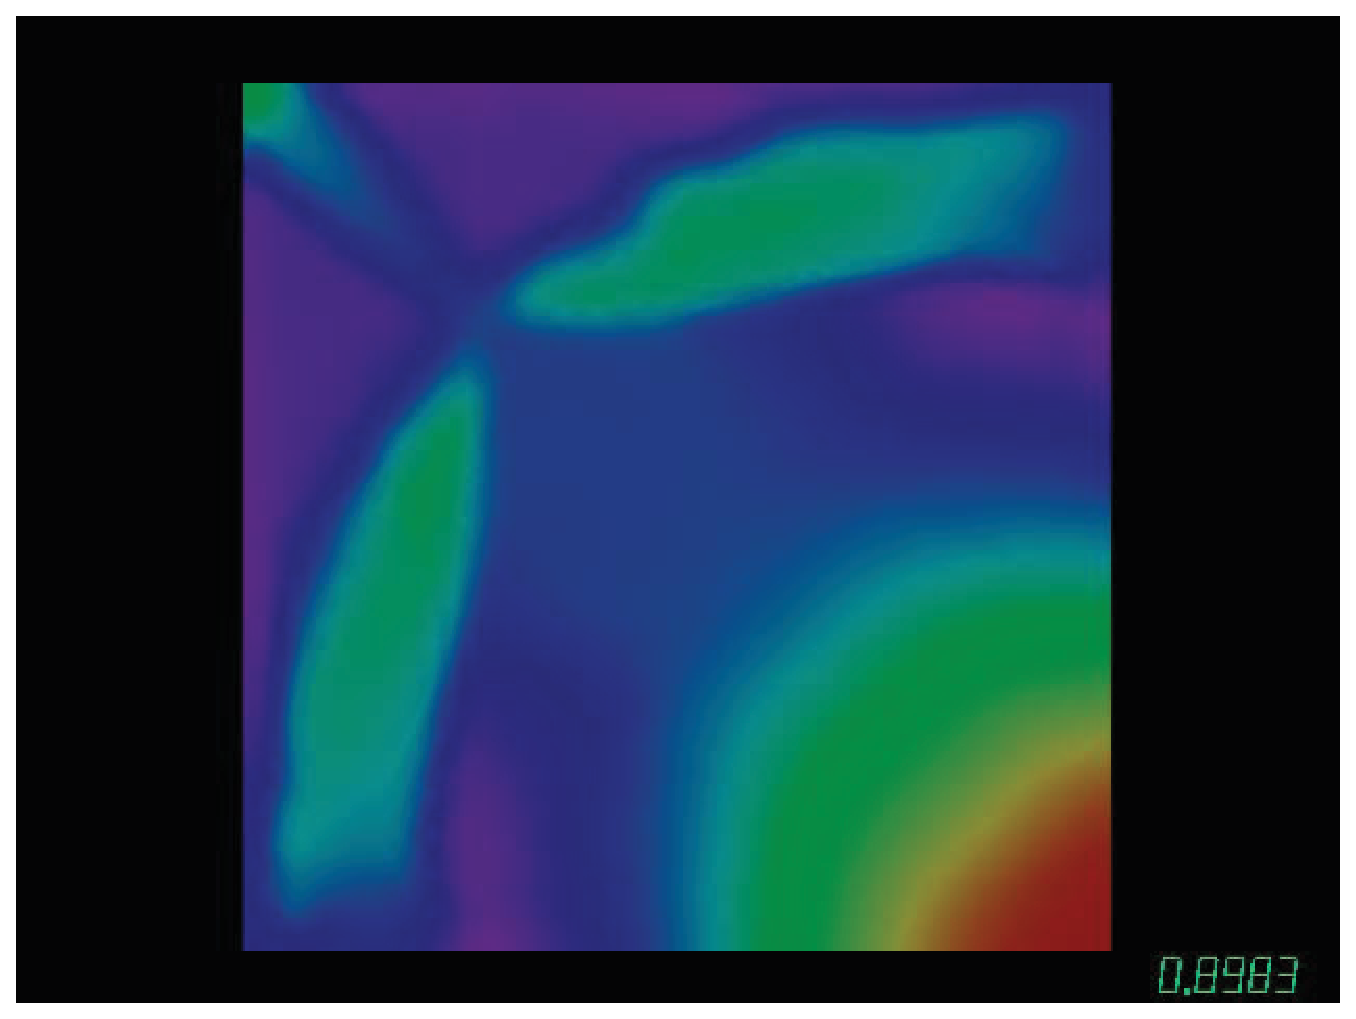
\includegraphics[width=0.8\linewidth]{Implosion}
\caption{Implosion test.}
\label{fig:implosion}
\end{figure}

\begin{figure}[H!]
\centering
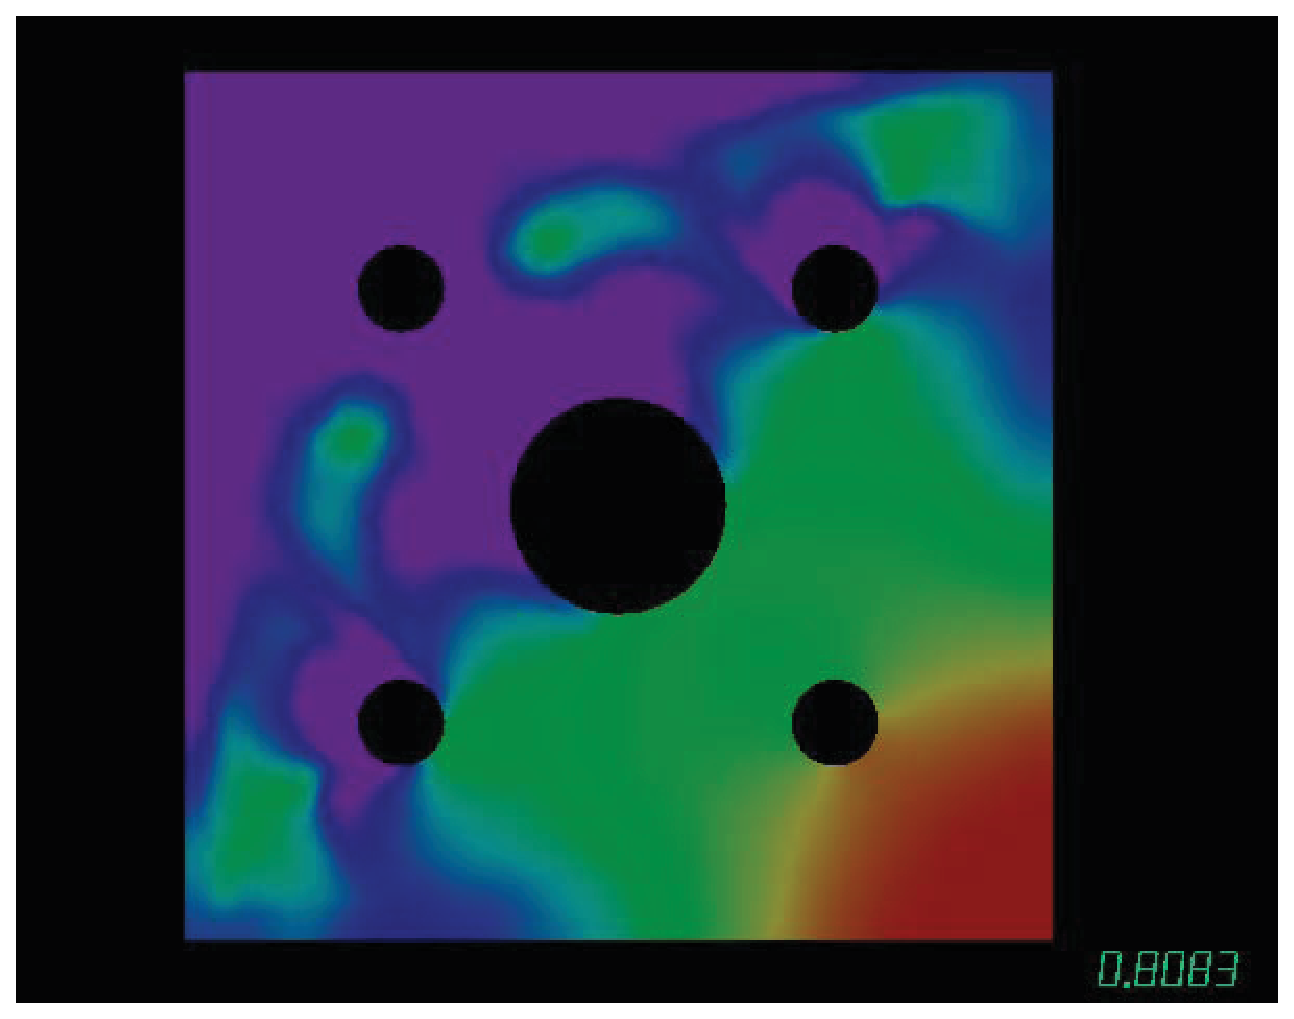
\includegraphics[width=0.8\linewidth]{ImplosionBear}
\caption{Implosion obstructed by obstacles.}
\label{fig:implosion2}
\end{figure}

\begin{figure}[H!]
\centering
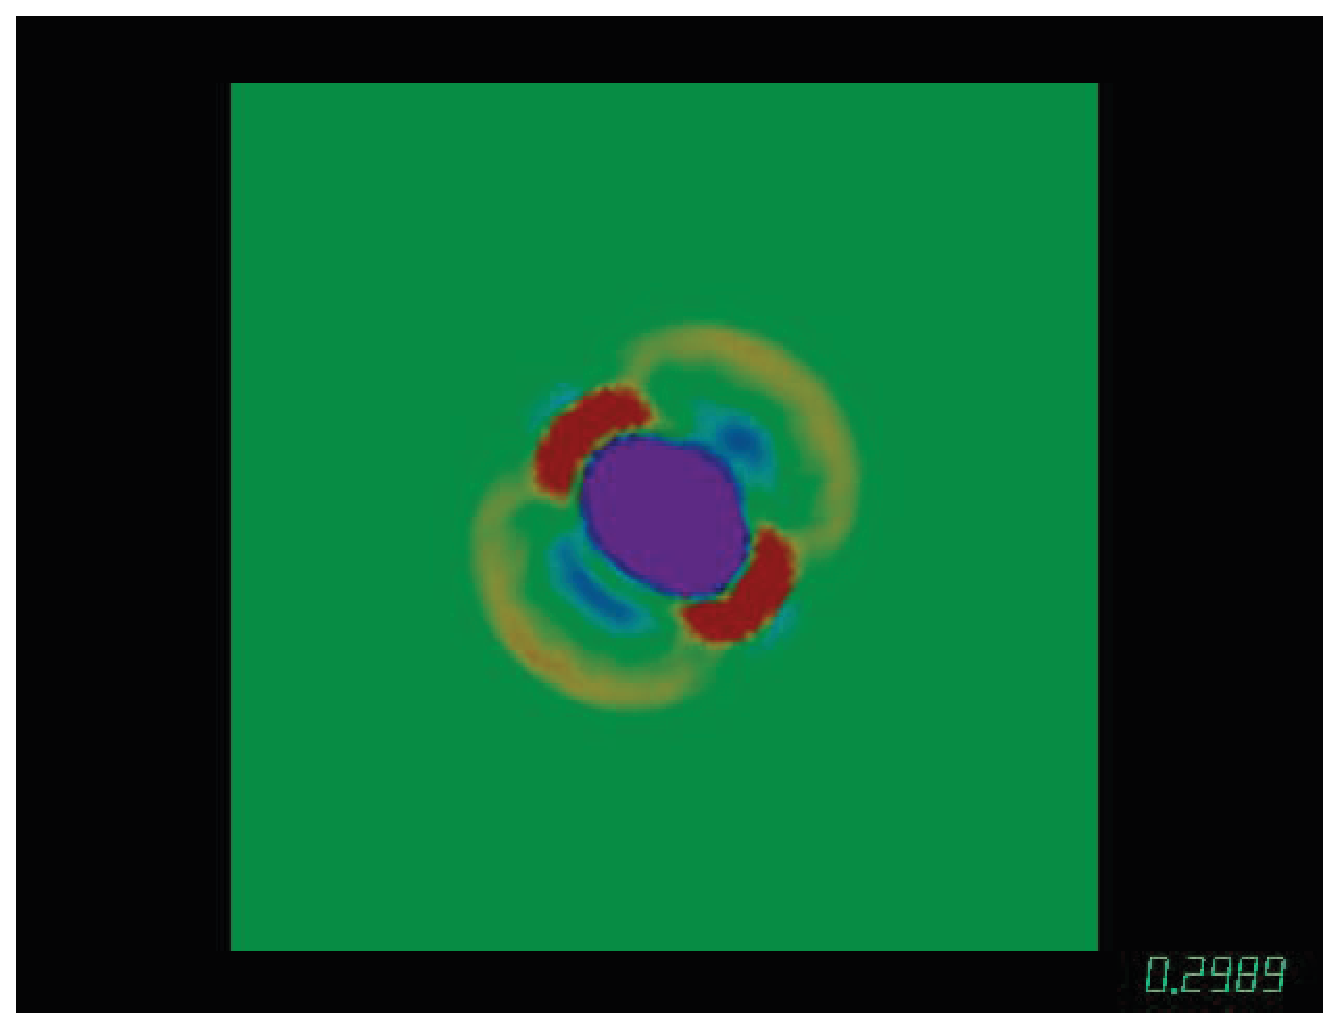
\includegraphics[width=0.8\linewidth]{BlastWave}
\caption{MHD Blast Wave test.}
\label{fig:blast}
\end{figure}

\begin{figure}[H!]
\centering
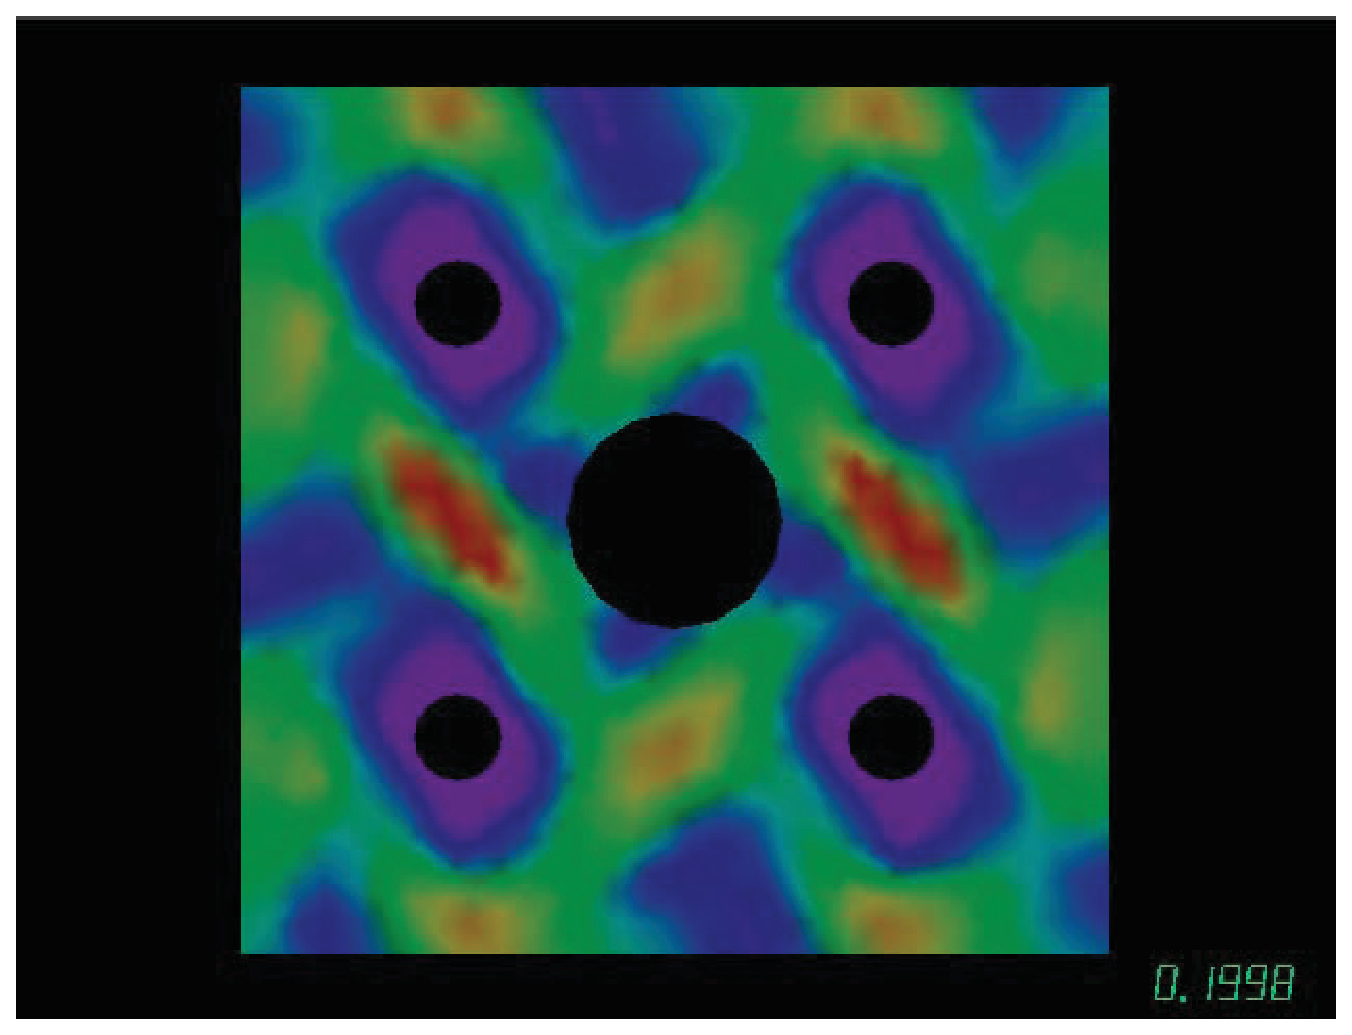
\includegraphics[width=0.8\linewidth]{OrszagTang}
\caption{Orszag-Tang test.}
\label{fig:ot}
\end{figure}

\begin{figure}[H!]
\centering
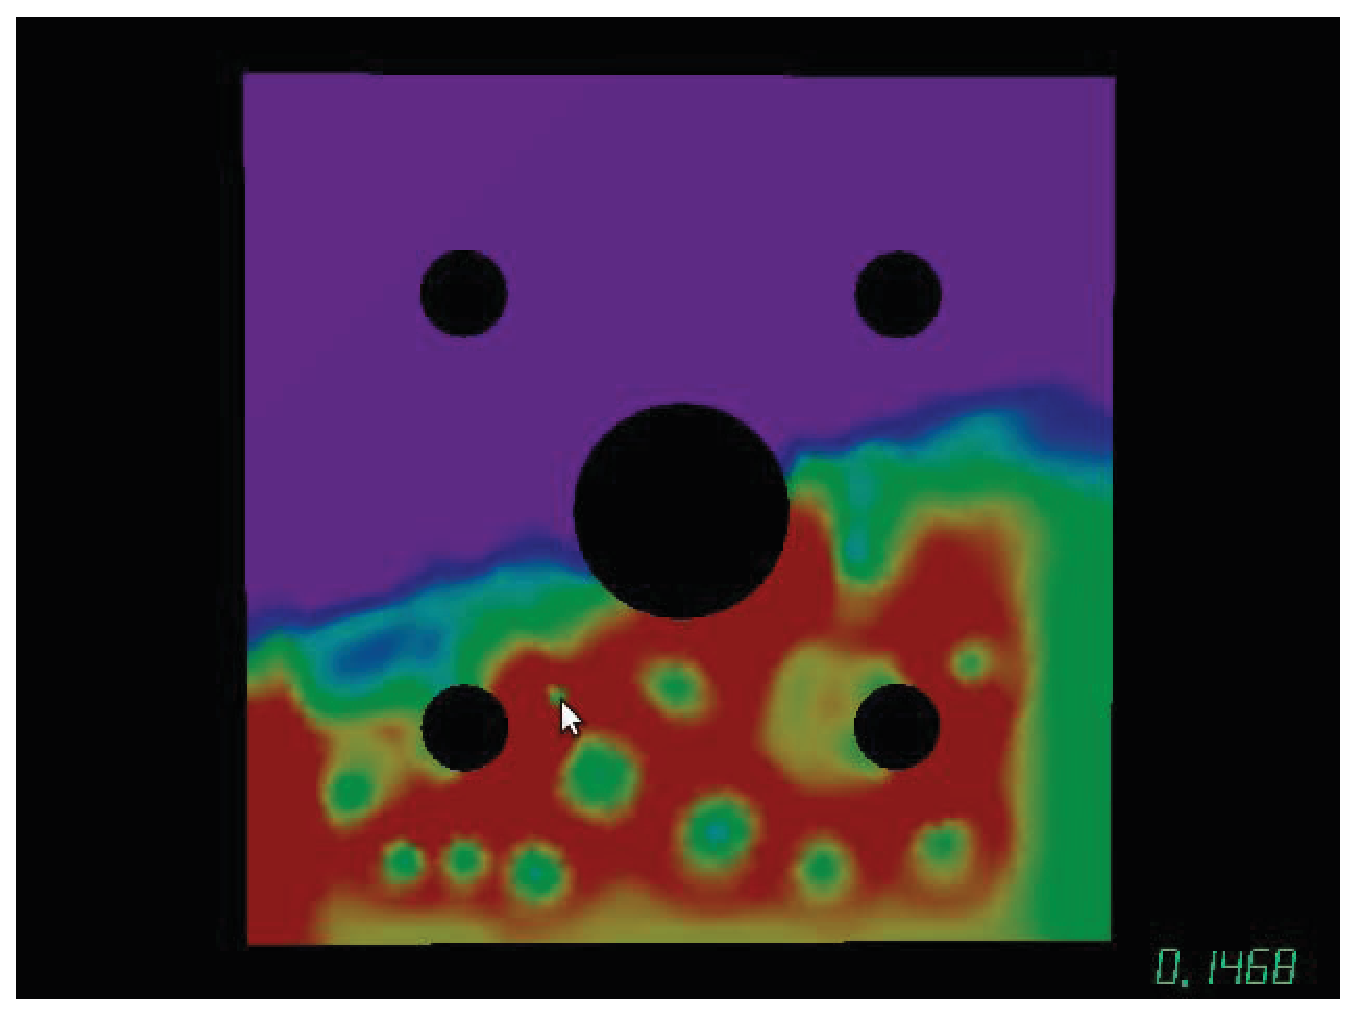
\includegraphics[width=0.8\linewidth]{HydroInteractive}
\caption{Screenshot of the 2-phase interactive fluid medium. The user has clicked at several locations to inject energy and set off blast waves.}
\label{fig:ih}
\end{figure}

\section{Examples from Running our Code}\label{sec:examples}

\subsection{Implosion}\label{sec:implosion}

Figure~\ref{fig:implosion} shows a screenshot of an implosion test, where a low density/pressure and high density/pressure interact to form shocks. Figure~\ref{fig:implosion2} shows the same setup, but obstructed by obstacles.

\subsection{MHD Blast Wave}\label{sec:blast}

Figure~\ref{fig:blast} shows a screenshot of a Sedov-Taylor like blast wave (energy injected at the center) evolving in a magnetic field at a $45$ degree angle. The density structure is elongated along the direction of the magnetic fields.

\subsection{Orszag-Tang}\label{sec:ot}

Figure~\ref{fig:ot} shows a screenshot of Orszag-Tang test for decaying supersonic magnetic turbulence with obstructions and reflective boundary conditions.

\subsection{Interactive Hydro}\label{sec:ih}

Figure~\ref{fig:ih} shows a screenshot of the 2-phase medium density field that the user has interactively set up and perturbed with injection of energy at several locations in the simulation.


\bibliography{mybib}

\end{document}
%###################################################################################################